\subsection{赤道全体での単調性の検査}\label{sec:radial-experiment}
根における下向きの交差以上のことを証明できるだろうか。形状を固定すると、数値的な動径曲線は、$H_\rho/\rho$が赤道全体で負であることを示唆する。元の被覆はこの主張を検査していなかった：$H$の正の下界が得られれば、それだけで箱は根の探索から除かれていたからである。そこで我々は、ただ一つの受理条件$E_{yyyy}<0$と、同じ導関数の二つの表示とを用いて、第二の実験を行った。$(\rho,0,0)$において$x=q_1$、$y=q_2$と書く。$\rho>0$に対して、式~\eqref{eq:fourth_derivative}を用いて二つの横断方向の固有値の差をとると、次を得る：
\[
 E_{yyyy}=3(E_{xx}-H)/\rho^2,\qquad H=E_{yy}.
\]
中心の近くでは、$\rho^2$による除算で情報が失われる。境界との接触の近くでは、元の曲面核を四回微分すると、視線距離の逆べきが現れる。我々は、$\rho\le 1/2$では直接の四階導関数を、$\rho\ge 1/2$では二つの弦Hessianの差を用いる。後者の表示に必要なのは、内点における二階導関数の有界な表示式だけである。結果は$0\le\rho<1$に関するものであり、$\rho=1$に達するパラメータの箱は、接触に任意に近い内点を被覆する。

\begin{figure}[htbp]
\centering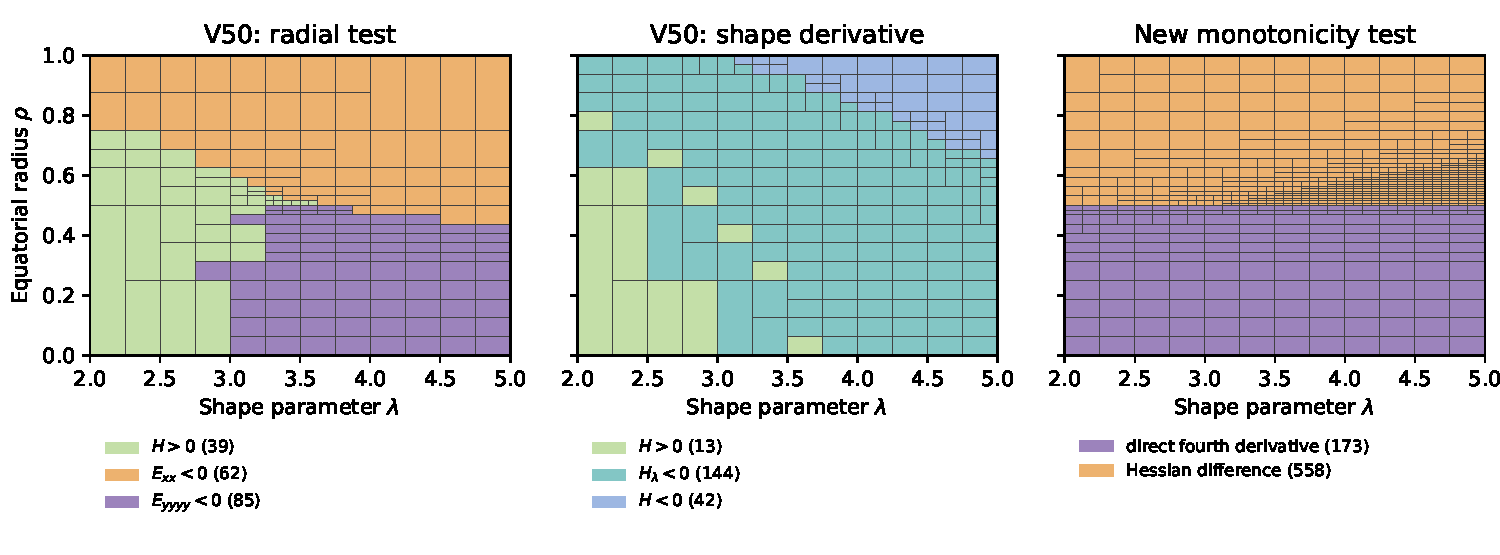
\includegraphics[width=\linewidth]{figures/gate_map.pdf}
\caption{完全に分割された三つの赤道上の検査における実際の終端長方形であり、凡例の数は終端の箱の個数である。最初の二つのパネルは、元の動径方向および形状方向の分割を再現する。三つ目は、ただ一つの符号についての新しい検査である。そこでの色の違いは、同じ四階導関数の二つの表示式を表す。}\label{fig:gate-map}
\end{figure}

\paragraph{記録された区間計算の結果。}
$[2,5]$上の幅$1/4$の十二個の形状スラブから出発した。新しい表には、直接の四階導関数の表示式に対する173個の終端の箱と、Hessianの差に対する558個の終端の箱が含まれる。半径の上端が$s$で半径の下端が正である外側の箱に対して、$H$の区間下界を$a$、$E_{xx}$の上界を$d$とする。$d<a$のとき、有理数$3(d-a)/s^2$は、その箱全体で$E_{yyyy}$の上界である。両方の種類の葉にわたる有理数の上端の最大値は次のとおりであった：
\[
             -109964349/2^{36} < -0.0016 .
\]
整数検査プログラムは、元の葉が出発時の各スラブを被覆することを検証する。第二の実装は、内側の箱では固定曲面エネルギーのTaylor係数を、外側の箱では弦方向における二つのHessian成分の差を積分する。これは元の箱の端点とモードを読み込む。全731個の箱において、局所的な細分の後、1,043個の小片上の上端の最大値は$-1/512$を下回った。したがって、どちらの実装からも上に示した上界が従う。補足ノートは、係数の公式、演算、および両方の被覆検査を与える。同じ元の検査を$1\leq\lambda\leq2$に拡張すると、176個の終端の箱（直接137個、弦39個）が得られ、上界は$-95257877/2^{36}$である。第二の評価プログラムもこれら176個の長方形を被覆し、399個の小片で、上端の最大値は$-0.00031$を下回った。この帯については、二つの独立な上界から、C3で用いる狭義の符号が従う。したがってこの帯では、記録された包囲が成り立つならば、C3における正の境界トレースから、赤道全体で$H>0$であることが従う。

\paragraph{記録された包囲が成り立つ場合の帰結。}
各$2\le\lambda\le5$に対して、$h'=\rho E_{yyyy}/3$であるから、関数$h(\rho)=H(\rho,0;\lambda)$は$(0,1)$上で狭義単調減少である。中心への連続性と、外側の端点における一階導関数のトレースへの連続性により、$h(0)>0>h(1)$ならば内部の半径がちょうど一つ得られ、そうでなければ一つも得られず、これは端点での値が零の場合も同様である。これが分類で用いる動径方向の一意性の議論である。縦方向の排除、二つの遷移の符号と位置、および半径の動きに対する$H_\lambda$は、別個の入力である。元の動径方向の実験には186個の葉があり、39個の箱が$H>0$を、62個が$E_{xx}<0$を、85個が$E_{yyyy}<0$を用いた。199個の葉からなる形状方向の被覆は、$H>0$、$H<0$、$H_\lambda<0$をそれぞれ13個、42個、144個の箱で用いた。これらの個数は実行時間のコストを比較するものではない。

図~\ref{fig:gate-map}において$\rho=1/2$のすぐ外側に箱が集中しているのは、表示の切り替えの位置で生じたものである。中心から離れた内部の重なりの上では、どちらの公式も利用できる。ここに示した計算は、$1/2$での固定した切断を用いる。
